\lecture{17}{24 aprile 2024}

\section{Produzione di onde elettromagnetiche}
Le sorgenti dei campi elettrico e magnetico sono le cariche. Consideriamo ua carica \(q>0\) ferma nell'origine che genera un campo elettrico statico. Questo non genera onde elettromagnetiche. Se mettiamo in moto la carica a velocità costante, esisterà un sistema di riferimento inerziale solidale con la carica in cui il campo elettrico è ancora statico. Le onde elettromagnetiche sono indipendenti dal SdR, quindi anche in questo caso non ho onde elettromagnetiche. Allora la carica deve essere accelerata! Divido l'asse dei tempi in tre fasi: carica ferma per \(t<0\), carica accelerata da \(0\) a \(\Delta t\) con accelerazione \(a\), carica in moto uniforme a velocità \(v=a \Delta t\) per \(t> \Delta t\). N.B.: per la teoria della relatività, esiste una regione finita centrata attorno all'origine in cui l'informazione sull'accelerazione della carica è arrivata. All'esterno l'informazione non è ancora arrivata. Quando la carica si muove di moto uniforme si ripete la stessa situazione: c'è una "bolla" che sa che la carica ha moto uniforme e una regione intermedia che non lo sa ancora.
\begin{figure}[H]
	\centering
	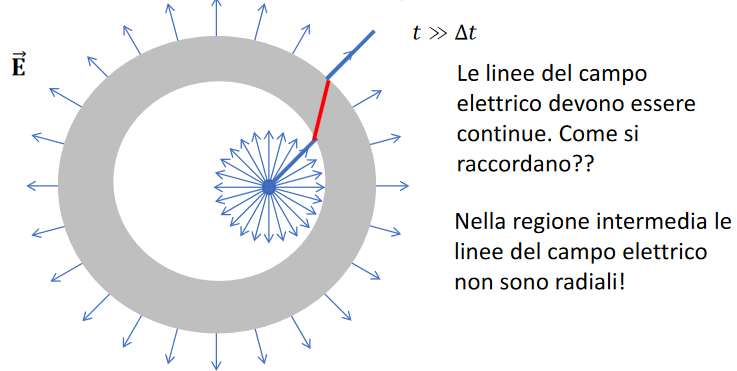
\includegraphics[width=0.6\textwidth]{screenshots/2024-04-24-09-25-42.png}
\end{figure}
\begin{figure}[H]
	\centering
	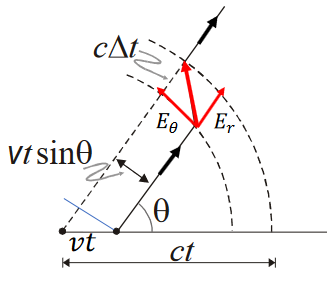
\includegraphics[width=0.4\textwidth]{screenshots/2024-04-24-09-30-00.png}
\end{figure}
Se \(v \ll c\), il campo \(\vec{E}\) si può raccordare con un segmento. Considero \(\Delta t\) piccolo a piacere e \(t \gg \Delta t\).
\begin{gather}
	\frac{E_{\theta } }{E_r} = \frac{vt \sin (\theta )}{c \Delta t} = \frac{a t \sin (\theta )}{c}\\
	\implies E_{\theta } = \left( \frac{q}{4 \pi \varepsilon _0 r^{2} } \right) \frac{a t \sin (\theta )}{c} \thickapprox \\
	\thickapprox \left( \frac{q}{4 \pi \varepsilon _0 r c t} \right) \frac{a t \sin (\theta )}{c} = \frac{1}{4\pi \varepsilon _0}\frac{qa \sin (\theta )}{c^{2} r}
\end{gather}
\begin{definition}
	[Campo di radiazione]
	Quanto trovato è detto "campo di radiazione":
	\begin{equation}
		E_{\theta } = \frac{q}{4 \pi \varepsilon _0}\frac{a \sin (\theta )}{c^{2} r} 
	\end{equation}
	Cala meno velocemente del campo elettrostatico, quindi a grandi distanze sarà più presente il campo di radiazione. Dipende anche dalla componente dell'accelerazione proiettata sulla direzione di propagazione del campo (\(a \sin (\theta )\)).
\end{definition}
Se ho un moto accelerato arbitrario, \(a = a(t)\). Il campo di radiazione impiega il tempo \(t_p =\quotient{r}{c} \):
\begin{gather}
	E_{\theta }(r,t+\frac{r}{c}) = \frac{q}{4 \pi \varepsilon _0} \frac{\sin(\theta )}{c^{2} r}a(t)\\
	E_{\theta }(r,t^{\prime} ) = \frac{q}{4 \pi \varepsilon _0}\frac{\sin (\theta )}{c^{2} r}a \left( t^{\prime} - \frac{r}{c} \right) 
\end{gather}
dove \(t\) è il tempo rispetto al moto nell'origine e \(t^{\prime} \) è il tempo visto dal punto in cui è presente il campo di radiazione. Un'accelerazione di breve durata implica un campo di radiazione impulsivo. Posso far oscillare la carica di moto armonico (\(y(t) = A \sin (\omega t) \rightsquigarrow a = \ddot{y = - \omega ^{2} A \sin (\omega t)}\)) e ottenere
\begin{align}
	E_{\theta }(r,t) &= - \frac{q}{4 \pi \varepsilon _0} \left( \frac{\omega }{c} \right)^{2} \frac{\sin (\theta )}{r} A \sin \left( \omega \left( t- \frac{r}{c} \right)  \right) =  \\
	&= A^{\prime} \frac{\omega ^{2} \sin (\theta )}{r} \sin (kr - \omega t)   
\end{align}
dove \(k \coloneqq \quotient{\omega }{c} \) e il tempo è quello nel punto in cui viene effettuata la misura. È, come previsto, un'onda sferica! L'ampiezza decresce come \(\quotient{1}{r} \).

\subsection{Dipolo oscillante}
Molto spesso le onde elettromagnetiche sono generate tramite dipoli oscillanti:
\begin{figure}[H]
	\centering
	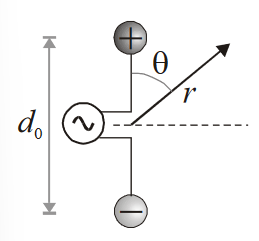
\includegraphics[width=0.3\textwidth]{screenshots/2024-04-24-09-54-08.png}
\end{figure}
Il momento di dipolo si scrive
\begin{equation}
	\vec{p} = \vec{p}_0 \sin (\omega t)
\end{equation}
con \(d_0 = 2A,\ p_0 = 2Aq\). Questo implica che possano oscillare le cariche a distanza costante o oscillare la distanza a cariche costanti. Lungo \(r\) si propaga un'onda elettromagnetica trasversale di intensità proporzionale al campo di radiazione:
\begin{equation}
	\langle I \rangle \propto \omega ^4 \frac{\sin ^{2} (\theta )}{r ^{2} }
\end{equation}

\subsection{Onda sferica}
L'onda sferica che si genera non è uniforme. \(E\) dipende dall'angolo \(\theta\). \(\vec{E}\) è lungo il meridiano, \(\vec{B}\) lungo il parallelo, la propagazione è lungo \(\vec{E} \cp \vec{B}\).
\begin{figure}[H]
	\centering
	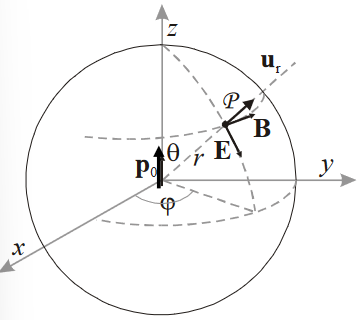
\includegraphics[width=0.4\textwidth]{screenshots/2024-04-24-09-57-28.png}
\end{figure}
\begin{figure}[H]
	\centering
	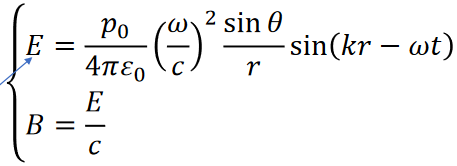
\includegraphics[width=0.5\textwidth]{screenshots/2024-04-24-10-01-06.png}
\end{figure}
Ho campi nulli lungo l'asse del dipolo (\(\theta = 0, \pi \)). È il motivo per cui le antenne WiFi poste in alto funzionano peggio e perché sotto un'antenna telefonica non prende bene.

\paragraph{Energia}
L'intensità può essere calcolata così:
\begin{figure}[H]
	\centering
	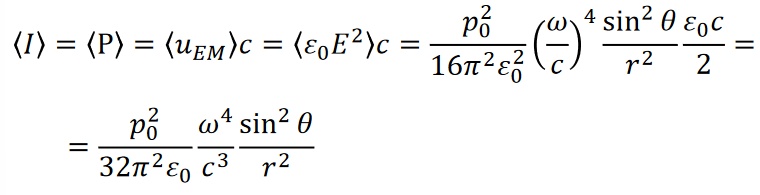
\includegraphics[width=0.5\textwidth]{screenshots/2024-04-24-10-02-48.png}
\end{figure}
Si può anche calcolare la potenza emessa da un'antenna:
\begin{figure}[H]
	\centering
	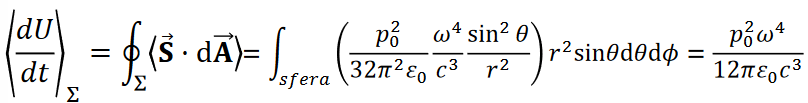
\includegraphics[width=0.55\textwidth]{screenshots/2024-04-24-10-04-00.png}
\end{figure}
Per raddoppiare la frequenza, è necessario aumentare la potenza di un fattore 16. Ci sono anche generatori di onde elettromagnetiche che funzionano con correnti oscillanti (quindi tramite un'induttanza che genera un campo magnetico variabile nel tempo). Si studiano nello stesso modo dei dipoli oscillanti tramite tramite la seguente analogia:
\begin{equation}
	\begin{cases}
		q &= q_0 \sin (\omega t)\\
		i &= \omega q_0 \cos (\omega t) = i_0 \cos (\omega t)
	\end{cases}
	\implies p_0 = q_0 d_0 = \frac{i_0 d_0}{\omega }
\end{equation}
che permette di modificare il contributo della pulsazione alla potenza:
\begin{figure}[H]
	\centering
	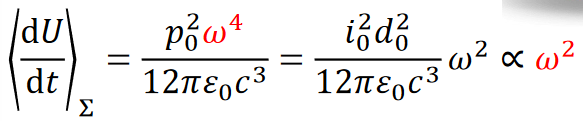
\includegraphics[width=0.4\textwidth]{screenshots/2024-04-24-10-09-39.png}
\end{figure}

\section{Spettro elettromagnetico}
Le onde elettromagnetiche sono principalmente descritte da tre grandezze: \(\nu = \quotient{\omega }{2 \pi } \) frequenza, \(\lambda = \quotient{c}{\nu } \) lunghezza d'onda, e \(E= \hslash \omega \) l'energia del fotone con \(\hslash = \SI{1.05 e-34}{J s} \). Lo spettro elettromagnetico è convenzionalmente diviso in 7 regioni:
\begin{figure}[H]
	\centering
	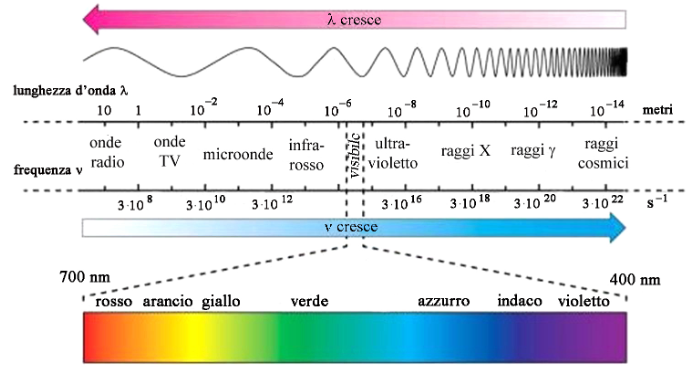
\includegraphics[width=0.5\textwidth]{screenshots/2024-04-24-10-30-49.png}
\end{figure}
Nelle onde radio (\num{0} - \SI{1}{GHz}) è difficile studiare la natura corpuscolare della luce. L'energia dei fotoni è molto bassa, quindi si tratta semplicemente come un'onda. Qui vanno la maggior parte dei segnali delle comunicazioni (radio, TV). 
\begin{figure}[H]
	\centering
	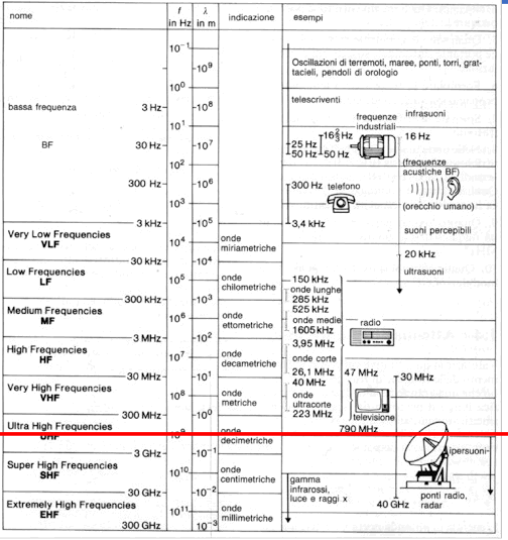
\includegraphics[width=0.4\textwidth]{screenshots/2024-04-24-10-38-17.png}
\end{figure}
Al di sopra delle onde radio si trovano le microonde (\num{1} - \SI{300}{GHz}). Il microonde funziona perché la molecola d'acqua entra in risonanza a \(\SI{2.45}{GHz} \). Gli spaghetti non si fanno a microonde. Le microonde sono usate per le comunicazioni dei telefoni cellulari, per il WiFi e per i radar che devono individuare gli aerei (se un aereo è lungo \SI{50}{m}, la lunghezza d'onda dev'essere molto minore).

Fra i \SI{0.3}{THz} e i \SI{428}{THz} si trova la banda dell'infrarosso. Qui si trovano le transizioni molecolari, l'emissione termica dei corpi e le comunicazioni in fibra ottica.

Tra i \SI{0.4}{\micro \metre} e i \SI{0.7}{\micro \metre} si trova la luce visibile. Qui risiedono le transizioni atomiche esterne (come lo spettro di emissione dell'idrogeno) e i colori. La descrizione deve essere necessariamente quantistica e quindi comprendere i fotoni. L'atmosfera è praticamente trasparente a queste onde elettromagnetiche:
\begin{figure}[H]
	\centering
	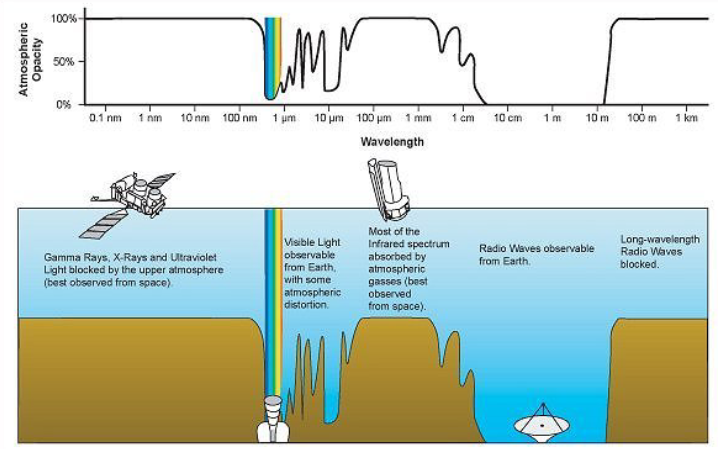
\includegraphics[width=0.6\textwidth]{screenshots/2024-04-24-10-44-59.png}
\end{figure}

La regione dell'ultravioletto è fra \SI{1}{nm} e \SI{0.4}{\micro \metre}. Qui avvengono le transizioni atomiche profonde.
\begin{figure}[H]
	\centering
	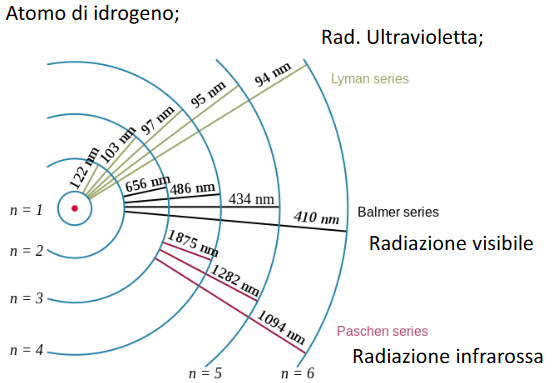
\includegraphics[width=0.5\textwidth]{screenshots/2024-04-24-10-49-54.png}
\end{figure}

I raggi X si trovano fra \SI{1}{keV} e \SI{100}{keV}. Non c'è identità di vedute su questo intervallo. Qui risiedono le transizioni atomiche profonde di atomi pesanti e il frenamento di elettroni. Vengono usati per le radiografie (trapassano la maggior parte della materia) e le cristallografie (studiare i reticoli cristallini).

I raggi gamma hanno un'energia maggiore di \SI{0.1}{MeV}. Le transizioni nucleari, le interazioni tra particelle elementari e i raggi cosmici appartengono a questa categoria. Nella figura seguente si vede il piano galattico studiato tramite raggi gamma:
\begin{figure}[H]
	\centering
	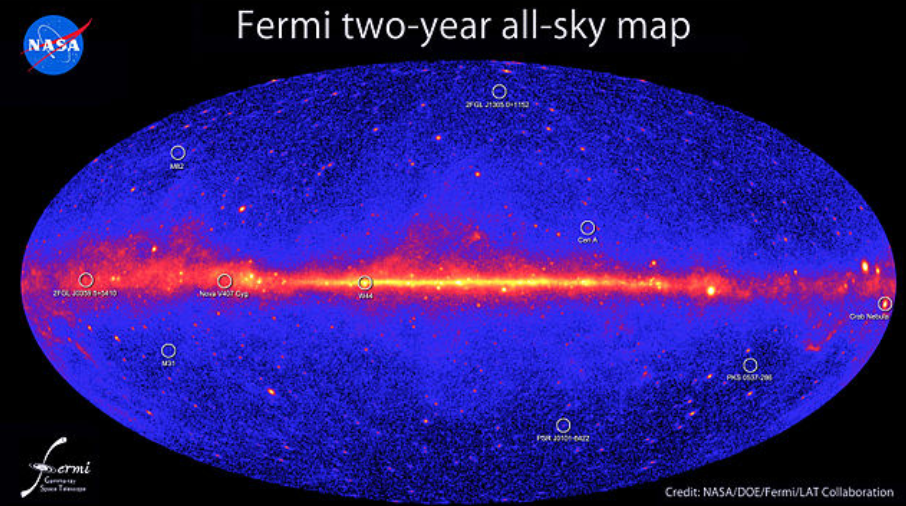
\includegraphics[width=0.5\textwidth]{screenshots/2024-04-24-10-57-52.png}
\end{figure}